\tikzsetnextfilename{externalized-shortest_path}
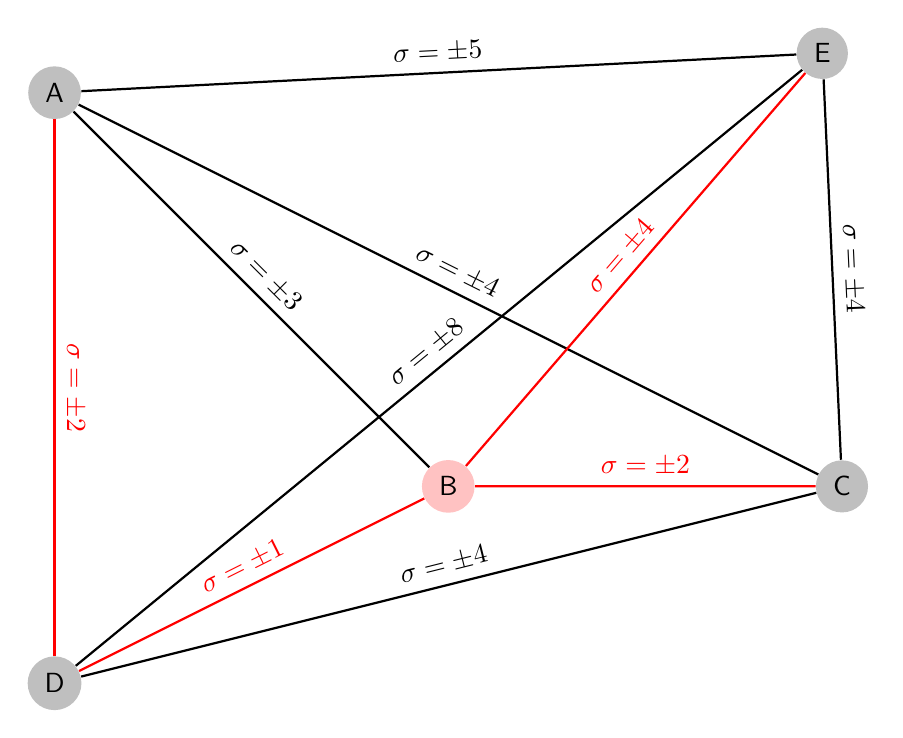
\begin{tikzpicture}
    [scale=2.5,
     font=\sffamily,
     vertex/.style={circle, fill=black!25},
     selected/.style={fill=red!24},
     edge/.style={draw, thick, -},
     short/.style={red}]
    % Draw the network
    % First we draw the vertices
    \foreach \pos / \name / \style in {
            {(0,3)/A/}, {(2,1)/B/selected}, {(4,1)/C/}, {(0,0)/D/}, {(3.9,3.2)/E/}}
        \node[vertex, \style] (\name) at \pos {\name};
    % Connect vertices with edges and draw weights
    \foreach \source / \dest / \offset / \error / \style in {
            A/B/7/3/,
            A/C/8/4/, B/C/7/2/short,
            A/D/5/2/short, B/D/5/1/short, C/D/6/4/,
            A/E/5/5/, B/E/5/4/short, C/E/6/4/, D/E/6/8/}
        \path[edge,\style] (\source) -- node[midway, above, sloped, align=left] {
          $\sigma = \SI{\pm\error}{\ns}$} (\dest);
\end{tikzpicture}
